

%\documentclass[man]{apa}
%\documentclass[doc]{article}{styles/apacls/apa}
\documentclass{report}


\usepackage{mathptmx}       % selects Times Roman as basic font
\usepackage{helvet}         % selects Helvetica as sans-serif font
\usepackage{courier}        % selects Courier as typewriter font
\usepackage{type1cm}        % activate if the above 3 fonts are
                            % not available on your system
\usepackage[utf8]{inputenc}
\usepackage{textcomp}
\usepackage{makeidx}         % allows index generation
\usepackage{graphicx}        % standard LaTeX graphics tool
                             % when including figure files
\usepackage{multicol}        % used for the two-column index
\usepackage[bottom]{footmisc}% places footnotes at page bottom

\usepackage{verbatim}        % per comentaris multilinia
\usepackage[utf8]{inputenc} %permite escribir {\'a},{\'e},{\'u},{\'o},{\'\i} & {\~n} directamente
\usepackage[british]{babel}
\usepackage{csquotes}
\usepackage{amsmath, amsthm, amssymb}
\usepackage{enumerate}

\begin{document}
\title{Coevolutionary strategies in MultiAgent systems. An approach using socionatural realistic environments.\\
\small{Master Thesis}}
\author{Alexis Torrano Mart\'inez}
\maketitle
\newpage

\pagenumbering{roman}
\begin{abstract}
The aim of this master thesis is the development of a multiagent model for a simulation  of two populations whose interactions are strongly influenced by a realistic landscape.
This research will be in line with Consolider-Simulpast (www.simulpast.es), an interdisciplinary project aimed to create simulations designed to be used in archaeological studies of human-environment interaction, decision-making processes and coevolutionary/competition behaviours of past societies.
The work plan will be focused on the development of first-stage models for two societies in the age of agriculture spreading surpasing the hunting and foraging way of living. The simulation will involve a climate engine for seasonality depending primarily on variable rainfall rate. Landscape information will be created from satellite image rasters. Constants, and variable relationship shall be modelled from measures and interviews with the experts. Data analysis tasks will be undertaken to validate the models and detect patterns in the archaeological record. Furthermore a comparison will be stablished between the classical simple models used in social simulation[1][2][8] and more advanced approaches.
\end{abstract}
\newpage 

\setcounter{tocdepth}{6}
\tableofcontents
\newpage 

\pagenumbering{arabic}
\chapter{Introduction}

\section{Description}

%Problem, Gujarat, Archeology (com al resum de la matri­cula).

\section{Motivation}

Simulation has been following an evolution in the models and paradigms applied to represent its target
systems. Dynamical systems, differential equations have been used and an overall simplification of the parts of the systems in the history of simulation to operate with the abstraction and simplification of the problems.
Mainly, reusing ideas from physical simulations, social sciences has modelled complex systems with dynamical
atomic entities that apply a simple set of centralized rules to move around the environment modelled. It was seen that due to the deeper details in human behaviour the question that could be solved and asked to that kind of models could not go very further as expected. 

To solve non-linearity phenomena, heterogeneity, hysteressis and other issues typical of complex systems, Agent Based Models(ABMs) where introduced to gain more insight of the modelled systems achieving good results. But under 
some conditions of very complex relationships between agents, highly specialized decission taking procedures
and issues in the environment led agents to need a sophysticated reasoning and problem solving capabilities
that are not specified and not yet introduced in ABMs coming from Social Sciences. 

We have found an example of that situation in our case study located in Gujarat from Simulpast project. Our agents must interact with a regular but changing environment to get resources, plan its actions, coordinate with its group and compete with other groups in a \textbf{co-evolution} dynamic. Because we want to find out why the Gujarat HunterGatherer(HG) way of life lasted more than in other place of Earth in its competition against AgroPastoralist(AP), we need to embed the behaviours of the survival strategies used by these groups. A simply reactive agent cannot cope with short term plus long term decissions in that competitive environment. So the question stated as topic for this Master Thesis project is \textbf{``do we get better results in social sciences simulations adding deeper AI techniques to make richer the behaviour or decission making engines of the entities in the system?''}. As we understand ``better results``, the outcome from the use of AI should be a more sound validation of the model, a nearier match of modelled behaviours with the real ones, and clearer, richer and robust scientific conclusions.

In order to study such posibilities Sugarscape[SugarScape] is a good framework to extend. Sugarscape is an artificial society developed by Joshua Epstein et al[Epstein]. where a number of inhabitants move to collect resources they need to live. Sugarscape models perception, lattice scanning in search of resources, sexual reproduction of the agents in the simulation, market relationships, immunology and spreading of diseases, and feature evolution. Epstein analises different experiments executed in the Sugarscape offering his conclusions and the dynamics emerging from the simulations. The results and conclusions will feed our AI experiments in order to make the comparisons of classical SugarScape agents vs AI agents, therefore, giving an answer to the topic of the Master Project.

\section{Simulation}

%brief description
%hi ha altres aplicacions de simulacio on no hi ha component temporal i no ho estic esmentant! MonteCarlo,etc...
Simulation is a discipline for performing virtual experiments in a computer. Computational techniques are used to build a model that represents your system. The dynamics of that system is codified in an algorithm that computes a calculus imitating the changes of state in the model, hence having a representation of that change along the time of the system modelled. Simulate is to play to ''what happens if...?'', and it is aimed to discover and explain the dynamics of a system to enhace or guide strategy development, decission taking, management, solving problems without analytical solutions or knowledge discovering and research. Although, we could get other positive benefits from it like theory checking or training through the inmersion in virtual worlds responding to our input.

% purpose, a priori, outcome,  { deduction, induction, abduction(Alexis) } Axelrod's
% crec que els agradara, marketing, saborcillo de IA impregnant els racons
A simulation obeys some direction of experimentation, so a question must be set to drive the selection of features to model from the real system and give a direction to the modelling and the experiments design.These assumptions choice will prune the details not related to the questions to solve. It is not just for the sake of simplicity but for the practical reason that a model too near of the real system will be as hard as the original system to analyse.\\
Simulation, like deduction, starts with a set of those explicit assumptions. But unlike deduction, it does not prove theorems. Instead, a simulation generates data that can be analysed inductively. Unlike typical induction, however, the simulated data comes from a rigorously specified artificial experiment rather than direct measurement of the real world. While induction can be used to find patterns in data, and deduction can be used to find consequences of assumptions, simulation modeling can be used as an aid intuition and hypothesis validation tool ( also as space search mechanism for parameter tunning or optimization ).
%abduction
Just like in a tipical Sherlock Holmes adventure you pick the evidences, scenario for the experiment, and the common knowledge (initial expert assumptions about the model). You enter in a refinement cycle where you test hypothesis and readjust them to discover the theory, the ``plot``, the explanation of what is happening. Following the abductive reasoning schema ... matching with SSSS needs...
%--: simulation, results, validation and statement of your inital hypothesis and question...
%--: simulation connected to abduction
% connect abduction with the simulation lifecycle 

Social simulation is a research field that applies computational methods to study issues in the social sciences. The issues explored include problems in psychology, sociology, political science, economics, anthropology, geography, archaeology and linguistics \cite{TakahashiSallachRouchier2007}.\\
Social simulation aims to cross the gap between the descriptive approach used in the social sciences and the formal approach used in the hard sciences, by moving the focus on the processes/mechanisms/behaviors that build the social reality.\\
In social simulation, computers supports human reasoning activities by executing these mechanisms. This field explores the simulation of societies as complex non-linear systems, which are difficult to study with classical mathematical equation-based models.
%reducibility 
Most of the times, studying complex systems implies to cope with non reducibility. One of the examples is Gravitational Dynamics. If our assumption is the use of Newton's mechanics, we can predict the state at any time or not, depending on the scenario. For a one dimension world you can predict the state at time $t_n$ from the initial state $t_0$ without computing all the preceding ones. For two and more dimensions you can only compute directly state $t_n$ if less the three bodies are implied. So in a real environment of many bodies in a 3D world you need to compute all the states from the initial to the one you consider as the last one. The system is non analytically reducible and you are forced to apply simulation to visit all the states and develop the behaviour of the model. It happens in most of the complex systems models, they have a nonlinear specification. Nonlinear models do not have a simple or computational reasonable analytical solution. 
% ( Classical Physics formulae used are non linear, acceleration is a quadratic factor in position <-- revisa aquesta fantasmada ) 

%emergence
Other of the main issues in complex systems simulation is emergence. While the initial assumptions may be simple, the consequences may not be at all obvious. The large-scale effects of locally interacting entities are called "emergent properties" of the system. Emergent properties are often surprising because it can be hard to anticipate the full consequences of even simple forms of interaction. 

%why simulation? because I need this non deducible emergence and the non deducible end state
There are some models, however, in which emergent properties can be formally deduced. Good examples include the neo-classical economic models in which rational agents operating under powerful assumptions about the availability of information and the capability to optimize can achieve an efficient reallocation of resources among themselves through costless trading. But when the agents use \textbf{adaptive} rather than optimizing strategies, deducing the consequences is often impossible; simulation becomes necessary.
% i ara estic preparat per conectar amb Social Science Simulation : reducibility + emergence forces to use simulation in S.S.

% Applying Simulation in the framework of Social Sciences to approach to the hypothesis of Simulpast targets, in concrete, about the case study from Gujarat, CS1.
%
%simulacio de sistemes complexes : f\'isica de particules, mercats, ... ecologia i... social sciences...
%
%n-body problem
%  2 body : formula
%  n body in 2D  : formula
%  n>2 body in 3D : simulation, non reducible
%   gravitation, electrostatics : input=initial position, output=end position, classical physics formulae: non linear!!!
%   acceleration is a quadratic factor in position!!!
%
%mes endevant cal caracteritzar la simulació : deterministic/stochastic, static/dynamic, open/closed, %linear/nonlinear, hysteressis, stable/unstable,
%stationary stage, emulation/monteCarlo/traceDriven/DiscreteEvent/DiscreteUnitTimeStep
%
%
%
%
\section{Question} 

% trobo a faltar m\'es xixa te\`orica, aix\`o s'hauria de semblar m\'es a un cap\'itol del Norvig.
In classical simulation approaches, specifically in the branch of Social Simulation, active entities which model human actors are designed with very simple behaviour engines. The classical hypothesis is that a complex mind for entities in the simulation are not that needed and maybe even could lead to difficult analysis of final results of the simulations (too daring statement?). 

Our statement is that, on the contrary, the mind engine of a simulation entity should not be bounded to that limit but special attention must be paid to give any necessary sofistication to give the entity a correct behaviour, real enough, sensible to the changes in the environment and competent to solve the issues that will have to solve along its lifetime in the system. Even more, we think that this entities' capability to respond with complex behaviours is the core that roots the modelling granularity needed to catch the essential of the social systems that we want to model.( a l'apartat de ABMs ho tornem a dir però afegint que cal adaptabilitat, resposta no lineal, aprenentatge depenent del temps, histeresis,...).\\
( i aixo motivaria els ABMs) Applying such premises we will explore the possibility to give or enhance decission
making, problem solving capabilities to the entities with the aim to get more accurate simulations and realistic models with higher matching against our job hypothesis and premises. We will take the framework of ABMs to integrate the AI techniques in a decission making schema of action-response dynamics sensible to a modelled world(por los pelos...).\\

%% ABM -> Decentralization of Decision-Making
\\
%%exposicio mes detallada dels punts febles que creus que trobaràs als simple agents (i a les conclusions 
%% d'AI-Sugarscape se't confirma 
%% i d'altres outcomes)

\indent \textbf{Do AI techniques contribute to better simulation results?}\\
\indent \textbf{Classic Simple Agent approach vs Rich Agents}\\
\indent \textbf{Did Gujarat extreme enviromental conditions delayed the HG disappearence?}\\
\newpage 
\chapter{Methodology}


% on poso el lifecycle del modelling procedure????
% specificacion --> expert's knowledge --> modelling --> prototipe --> { accept model | go to a previous state }
% revisiting early stages to refine models : toy model --> reviewing your assumptions about the main purpose
% interviews and ecotono meetings to motivate and help knowledge extraction
% ecotono modellings as a means to gain insight of the problem and the system, inspirational ideas.


\section{Intro}

%% metode = modelling\\
%% tecnica en ciencies socials = ABMs \\
%% afegir capitol llibre Rub+Cris\\
\\
%que es modelling en ciencies socials 
\\

%%% XR
%%Computer modelling and complex systems simulation have dominated the scientific debate over the last decade, %%providing important outcomes in biology, geology and life sciences, and resulting in the birth of entirely new %%disciplines (e.g. bioinformatics, geoinformatics, health informatics, etc.). In the social sciences, the number of groups currently developing research programs in this direction is increasing. The results are extremely promising since simulation technologies have the potential to become an essential tool in the field \cite{Gilbert2008}.\\
%%However, some social scientists are sceptical about the idea of reproducing “inside” a computer population dynamics, because of the perceived complexity of social structures. This scepticism is understandable given the low number of projects that used this approach and the lack of experience of social scientists with these tools. Nevertheless, the research done in complexity science during recent years shows the way computer simulation can be applied to this field. Artificial intelligence portrays how the appropriate interconnection of very simple computational mechanisms is able to show extraordinary complex patterns, and access to distributed computing has become affordable. For this reason, agent-based simulation allows the implementation of experiments and studies that would not be viable otherwise \cite{Pavon2008}. \\

% ATM mini intro
Modelling is a widely extended methodology. It comes from the natural observation of the world and the curiosity or need to reproduce it.\\
Modelling will be our framework for communication between archeologists' and sociologists' knowledge and their conceptualizations with our formal representations from computer science practices( simulation, algorithms, AI ).
The reason is that it is a procedure that will help to communicate the \textbf{discursive} nature of Social Sciences with the formal structures from Computer Science. The enginering of model development will allow us to reach a connection from experts' knowledge to a model that comprises the set of detail clearing out the ambiguity that language could filtrate. Also, the model development cycle will help set a picture of the system without inconsistencies, with each fact sound,  coherent and consistent from the logical point of view with the whole. 

\section{Why model}

% ATM, que es modelar? i com es modela?
The modelling process consists in identifying separable entities, processes, relationships and any rellevant information related to the question to solve and the domain of study. Indeed just thinking about something implies an unconscious projection of our mental frame hence producing a set of concepts and relationships that give birth to a model. The missed step is that it was not made explicit through some formal representation. A model is a logical and conceptual prototipe.
As Epstein \cite{Epstein2008} says \textit{“Anyone who ventures a projection, or imagines how a social dynamic—an epidemic, war, or migration—would unfold is running some model”}.\\

Modelling is an introspection exercise where you take into account the domain to elaborate a \textbf{formal} representation of the conceptualizations you develop around the problem. Mainly, it will have to do with mathematical expressions from calculus or algebra and logics. That is called \textbf{conceptual modelling}. This phase comprises the development of a relevant simplification, which must be complete according to the phenomena that inspires the question. Anything left out will change the outcome of the simulation, and non-relevant added items will produce noise that will difficult posterior analisys. All the involved facts must be correctly well grounded taking into account that any unneeded compound in the model will also be added to the scientific and mathematic justification, adding good-for-nothing effort. \\

For instance, I am modelling the dynamics of a restaurant to find an optimum allocation of waiters between interior and terrace tables and their serving policy, so I could minimize hired waiters while lowering the waiting time of clients. Variables like client arrival rate, kitchen serving time, number of interior tables, number of terrace tables are reasonable parts of the system to add to the simplification. The colour of the courtains, the outfit of the waiters most probably will not account for the stated optimization objective. Someone could argue about the topology of the tables whether it should be added or not to the model. But if I would model the system to analyze the survival rate when there is a fire and people must exit from the building as soon as possible, table and furniture topology is an unquestionable variable.\\

This kind of criteria should lead to a preference for simpler models. There are many reasons which force to design consciously with this premise. More complex models require harder effort to work their credibility, verification for the correct implementation of the conceptual model, and from the formal point of view, validation of the model and the scientific conclussions. Considering the system conceptualization and formalization, a more complex model is more open to criticism for the objective or subjective choice of features and modelling decisions. Why the present features were chosen and the missing ones were left out? why one expert point of view, and not other one? Also, as Robinson \cite{Robinson2008} states, simple models have many advantages, such as they are faster, require less data, are more flexible and, more importantly, if we better understand them we can better interpret their results. The KISS Lemma sumarizes it ``Keep It Simple, Stupid''.\\

% ATM:aqui o mes endevant? aprofondir molt?
Another concern is that detail and granularity choice is attached to the overall direction that takes the construction of the model in terms of structure. At this point it is interesting to mention how does a model can be grown.\\
The theory describes the domain as an ontological corpus of interelated conceptualizations where the pieces of knowledge can be related with equal to equal or relationships of subsumption and hierarchical connection. Following the distribution induced by such hierarchy the space of conceptualizations of the theory will have bounds in the higher and deeper concepts found in the top and bottom locations of the hierarchy. Usually, modelling methodology takes either the top, bottom or a midle layer to crystalize the model following the hierarchy in a direction towards the higher concepts or the deeper. An ascending crystalization is called \textbf{bottom-up} and the inverse direction is known as \textbf{top-down}. Crystalization could begin in a midle layer and stop before arriving a top or bottom bound layer. But can also happen that the modelization requires go further the bound. For instance, consider we are modelling a society to see the emergence of some differentiated groups. We could model towns, neighbourhoods, go down to families and then arrive to the person. Maybe we would like to characterized persons to some inner features related to their personality; now we are entering in a layer belonging to psychology sciences, we have surpassed the bottom conceptualization in sociology. If we go further we could arrive to the brain structures entering the field of neurology. We could continue to mollecules, biochemistry, and so on and so forth.   

%%% TODO posar dibuix : triangle, 2 fletxes: top->dw, bott->up
%%% analisys of system
%%% synthesis
%%% sometimes you do a mix


%George Box
Although good modelling of the parts could be accomplished lefting out the non-relevant phenomena, citing the famous quote of George Box, essentially, all models are wrong, but some are useful.\\

% multidiscpl ATM
As said before, Social Sciences represent their knowledge in discursive texts using natural language. In our Gujarat project we are experiencing interaction between different disciplines of social sciences : anthropology, archeology, and sociology. Each one of these branches has its own terminology, target problems and argue their discurse with different structures. 
Besides having to cope with implicit ambiguity in each discursive knowledge, all these branches must cooperate in a common framework connecting the different used conceptualizations. Some branches can organize their knowledge in concepts of entities, other use processes or actions, for instance. We cannot collapse this frameworks directly in a formal model. The modelling process will ellicite this structures and will match them with the mathematical tools offered by the chosen paradigm( lets say Dynamical System Theory, Agent Based Models, Petri Nets ). We will translate the conceptualizations to a common language that will connect the formalizations in a whole, the \textbf{conceptual framework}.  
Modelling will help to find a consensus for expressing the concepts and properties, will help to ellicite knowledge, arrange ambiguities, detect common points. It will allow as to embed the needed rigor to work under the same framework to make every part work together ( aixo sona fatxa i centralista :P ). Modelling shall be an exercise of shared development that can approach positions and circle a communication problem to solve the issues that will arise.
% posar les 2 figures de multidiscp modelling

%%%ellicitation 
%posar l'exercici de comprensio entre BSC - IMF, elicitation, ecotonos...? o deixar-ho per capitols posteriors?


%models que es contraduien-- camp de la física p.e.

%tradició de modelat en ciències socials

\section{Modeling in social sciences}
\label{sec:modelsinSC}

%%%% content

%society/social sc descrip, 
Social Sciences study the outcome of the interaction of individuals, the behaviour of society or distinguishable
groups inditified in it. The study of society or social groups considers its target as a adaptative ecosystem of people with interaction, other living entities, environmental conditions or environmental dynamics, information
exchange and the mutual adaptative changes induced between the actors, co-evolution.

%modelling targets/items, 

Modelling societies implies being aware of constituents identified by the social theories. Interacting entities conform a society. Such entities are observed and abstracted from identifiable individuals, people, and activity units, for instance families, neighbourhoods or job partners, composed also of the same individuals. 
An individual leaves a trace of participations and interactions in the society. Such activities occur with other
individuals, with some activity units or through them. Populations of individuals flow through the social structures, selectively participating and differentially performing. 
Ordinary living involves a participation of people in the social activities of family, leisure and holidays, shopping, work and travel. Activity within a unit is structured by relationships and choices, rules, rituals and randomness. Ordinary living also involves the participation of cultural ideas and artefacts in social activities.\\
The social sciences seek to understand not only how individuals behave under the social influence, but also how the interaction of many individuals leads to large-scale outcomes and global phenomena. 
%%
The main issues observed, individuals, units, processes or actions, flow and dynamics within units, are the frontline of the modelization aspects and motivation for the different paradigms appeared or adapted to solve the modeling objectives. New knowledge to infer from this identified phenomena will be the \textbf{descriptive} statement of observed behaviour, quantitative empirical \textbf{generalisations}, construction or assesment of \textbf{theories} and \textbf{prediction} models.

% reproducció parcial, ilegal?
\begin{figure}[tp]
\setlength\fboxsep{0pt}
\setlength\fboxrule{0.5pt}
\fbox{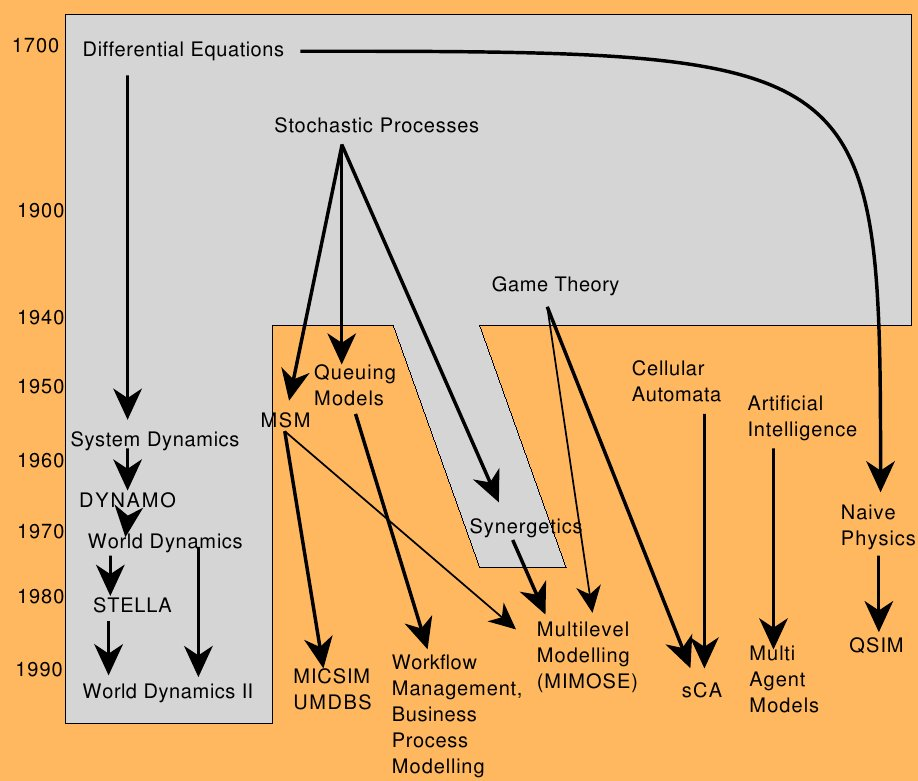
\includegraphics[width=120mm,keepaspectratio=true]{figures/Gilbert_pg21.jpg}}
\caption{The development of contemporary approaches to simulation in the social sciences (after Troitzsch 1997)}
%by Gilbert \cite{GilbertTroitzsch}}
\label{fig:SimTL}
\end{figure}

%possible paradigms. TOASK : Explico mes que son sistemes dinamics i la resta d'opcions?????

The first paradigms to model social processes were borrowed from the fields of physics, operations research, and economics materialized as game theory. The first social concepts considered were those related to social units or subgroups and large processes. Also, due to the main use of dynamical systems and differential equations, social phenomena was modelled as a flow between different containers that represent groups or state of individuals.\\

\begin{figure}[tp]
\setlength\fboxsep{0pt}
\setlength\fboxrule{0.5pt}
\fbox{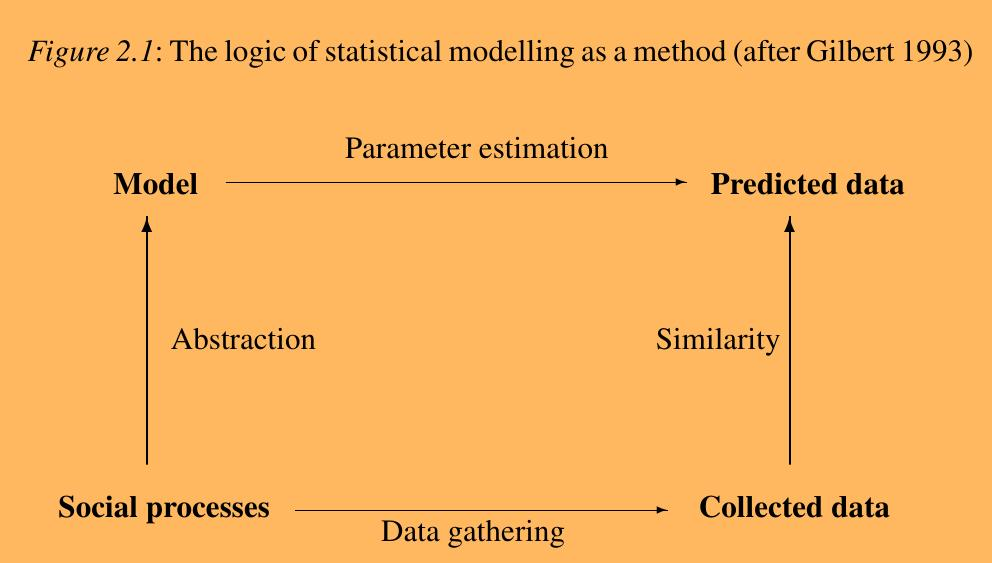
\includegraphics[width=120mm,keepaspectratio=true]{figures/statisticalModelling1.jpg}}
\caption{The logic of statistical modelling (after Gilbert 1993)}
%by Gilbert \cite{GilbertTroitzsch}}
\label{fig:SimTL}
\end{figure}

Richer representations to cope with reality led to nonlinear specifications and the introduction of heterogeneity present in social systems making them hard to represent or analitically unsolvable, hence, the following years saw the spreading of \textbf{simulation techniques}, first AI aproximations, cellular automatas and Petri's networks that allowed a finer granularity going from the top abstract groupings infered in social theories to the individual entities.\\

Gradually social modelling began to approach computational sciences keeping its connections to mathematics and statistics. Programming languages are more expressive, less abstract than most mathematical techniques. Programs deal more easily with parallel processes and processes without a well-defined order of actions compared to math equations. There is a quite long experience on studying programs and their properties from Algorithmics, Soft Engineering, and Operating Systems. The enginering of big models benefits from these branches endowing them with the desirable properties of modularity, extendibility, the experience of combining programs to grow huge program systems, error detection and maintenance, to mention some.

\begin{figure}[tp]
\setlength\fboxsep{0pt}
\setlength\fboxrule{0.5pt}
\fbox{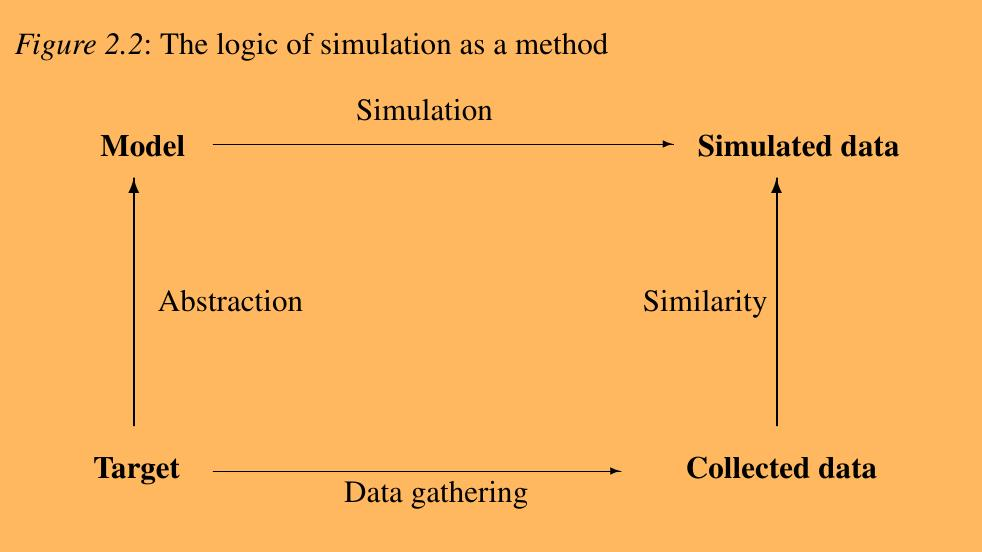
\includegraphics[width=120mm,keepaspectratio=true]{figures/simulationModelling1.jpg}}
\caption{The logic of simulation as a method (after Gilbert 1993)}
%by Gilbert \cite{GilbertTroitzsch}}
\label{fig:SimTL}
\end{figure}

%non covered issues that motivate ABM, 
%TOASK separo més l'explicacio? part1: primers pseudo-agents part2:agents 100%, propietats aconseguides...
This last improvement and the use of MultiAgent Modelling in social modelling allowed to introduce the bottom layer of the hierarchy of concepts of social science, \textbf{people} and all the package of phenomena and issues associated to it. Once you are modelling a person you can work directly with personal or social relationships and their properties, arity, creation and destruction mechanisms, transitivity and interaction rules. This allows to solve models non solved before, like some cooperation, coordination and competition scenarios from game theory where several agents are involved, for instance. Also the direct interaction and feedback effects between the entities and the  environment can be represented in the model. Before this step, other paradigms could not cope with the intrinsic phenomena of people interacting in a social scenario. Different issues had to be modelled, agent decission process modelling and embedding of the Rational Choice Theory, heterogeneity in the entitites, bounded rationality, and complex psychology.\\ 
Modelling from a bottom-up point of view with the inclusion of agents will allow to be near the real causes of macroscopic large scale phenomena non predicted from the microscopic local issues. Complex systems theory calls this \textbf{emergence}.
A further section will describe this effect.

% per on poses aixo? : ``Richer representations to cope with reality led to nonlinear specifications and the introduction of heterogeneity present in social systems''. 
 

%% ******* Modeling Lifecycle: SDLC; TOASK caldria una explicacio? nomes un grafic?
%% no diguis Lifecycle, es Methodology

Modeling methodology will be materialized through the framework of simulation technique. It will follow a series
of stages defined in simulation-based research. 

\begin{description}
\renewcommand{\labelitemi}{$\bullet$}
\renewcommand{\labelitemii}{$\cdot$}
\item [Definition of the target] A purpose for the model o a question over the target system is stated.
	\begin{description}
	\item [prediction/prognosis]
	\item [diagnosis]
	\item [theory validation / discovering]
	\item [study future possible worlds]
	\end{description}
\item [Observations] Data gathering, parameters and initial conditions retrieval from the target system using bibliography, interviews and experts' supervision.
\item [Assumptions] Relevant simplifications are considered. 
\item [Design model] Translation of the experts' conceptualizations to a formal modeling language or structure. 
\item [Computer programming] Implementation of the model.
	\begin{description}
	\item [verification] Test that the program matches the specifications and features of the formal model.
	\end{description}
\item [Run simulation] Perform the experiments.
\item [Gather results] Extract conclussions from the simulation data. 
\item [Validation] Check that the conclussions are scientifically sound and match the plausible target system behaviour. The model should behave similar to the target system under the selected features and details.
	\begin{description}
	\item [sensivity analisys] Detect variables and parameters that produce great oscilations on the simulation results.
	\end{description}
\end{description}


\begin{figure}[tp]
\setlength\fboxsep{0pt}
\setlength\fboxrule{0.5pt}
\fbox{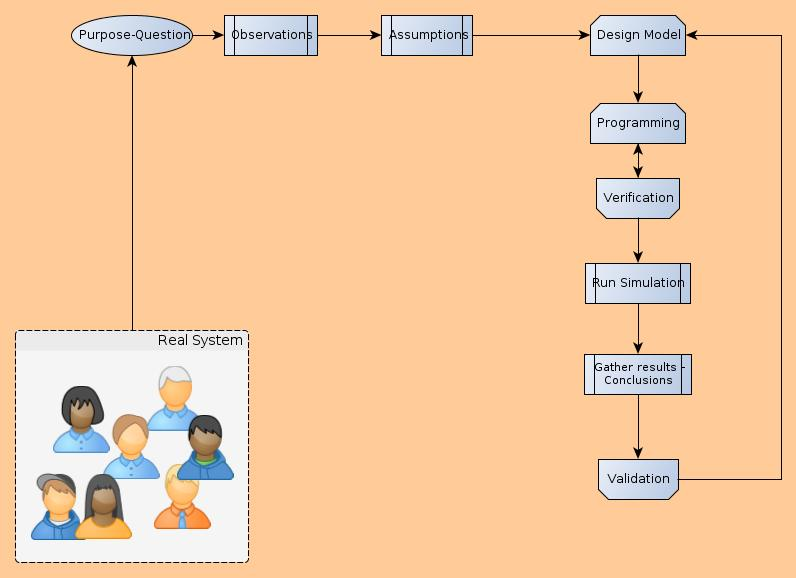
\includegraphics[width=120mm,keepaspectratio=true]{figures/simulationMethodlogy.jpg}}
\caption{Stages defined in simulation-based research (after ... )}
%by Gilbert \cite{GilbertTroitzsch}}
\label{fig:SimTL}
\end{figure}


%% Emergence
%Understanding a political or economic system requires more than an understanding of the individuals that comprise the system. It also requires understanding how the individuals interact with each other, and how the results can be more than the sum of the parts.

%bridge to ABM section

%%%% end content


% TOASK afegir certs apartats de l'ODD??? adaptar les descripcions dels apartats de l'ODD\\

%Comp emergent

%%%%%%%%%%%%%%%%%%%%%%%%%%
\section{Conceptual Framework}

\subsection{Multi Agent Systems}

%% aqui poses tota la part mes tecnica/teorica dels agents, a ABM ja no caldra explicar-ho
%% ABM explicara issues de modelatge i aplicacio cientifica

A MAS is build from some atomic identified entities in a bottom up design procedure.\\
Such entities are active decission making actors in the modelled system. The modelling lifecycle of an MAS will consider a stage where decission making processes must be identified from the system. Usually that decission making 
actions are carried along by more or less clear individual entities from the system. The modelling process will take the task to set the matching between these entities and the agent that will conform the MAS. The concept 
'' agent '' condenses a set of features that will specify the modelling metaphor that an agent represents:
some enclosed set of mechanisms to be aware of the state of the system, a set of goals to accomplish and the engine to decide from a bounded perception of the world, the actions to apply on it to achieve these goals. Besides the reasoning component of the agents, MASs have a strong component of inter-agent relationship. How one agent interacts with other agents could as important or more as how it reacts to world changes.
\\
bottom-up approach, reductionist way of looking at the things, we try to understand the parts\\
to join them from their relationship and then we try to get the big picture.
\\

al conceptual framework : parla dels conceptes, que venen de MultiAgent systems...
a la section d'ABM continua contactant amb MultiAgent Systems

\subsubsection{Agents}

agent -> metaphor ( agrada a l'Ulisses)

---------agents, una component que dispara la no linearitat i per tant la complexitat\\
---------heterogeneitat : dos \`atoms de Carboni es comporten igual en mateixes condicions, les persones no.\\

		Features:
\\
		  agents ( els features isolats )
		    goal planning/seeking
		    reasoning
		    adaptation
		    decission making
\\
		  social interaction
\\
		  emergence
		    complex behaviour patterns arising from goals and social interactions.
		    counterintuitive patterns : example of the colum in front of the exit door.
\\		    
		  bottom-up modelization
		    identify reasoning/deciding units : what will become agents
		    identify agents' relationships. 
\\
		  natural correspondence/matching of identified entities in social systems vs 
		  agents in the ABMs theoretical framework
\\
		  temporal correlation - histeresis
\\
%%%%%%%%%%%%%%%


\subsection{Complex Systems}
\subsection{Coevolution}
\subsection{Emergence}

Emergence is the outcome of the parts of the system that due to the dynamics of the intearactions of these parts. Emergence cannot be predicted from only the constituents and their addition, the feedback must be taken into consideration. Emergence is a global effect produced by local dynamics. 
%Exemple de la columna i una altre que sigui de social sciences...
The Column example.\\
There is potential for emergent phenomena, i.e., when
\begin{itemize} 
\item Agent behaviour is non linear ( weight sum of variables), or is expressed with discontinuities, if-then rules in a categorical framework or in discrete non continous manner.
\item Under memory phenomena, path-dependence, and hysteresis, non-markovian behavior, or temporal correlations, including learning and adaptation. 
\item Heterogeneous interactions between agents.
\item When there is unstability to perturbations although the system could be defined linearly.
\end{itemize}


%%%%%%%%%%%%%%%%%%%%%%%%%%%%%%%%%%%%%%%%%%%%%%%%%%%%%%%%%%%%%
\section{ABM}

%% definition - description

ABM is a modeling methodology that relies on a application engineering architecture called Multi Agent Systems from A.I.
 
Following the paradigm of ABM, systems to model are decomposed into entities called agents, which have their behaviour defined,  how affect or are affected by environment, and how they interact with the other agents. The main activity for agents is decision making. Each agent individually assesses the current state of the environment, taking into account the other agents, and in accordance with its objectives takes an action that runs against the system, the environment plus the agents that may be involved. The system runs on a constant loop of evaluations, decisions and actions of the agents that inhabit it.
This will lead to situations of iterated interactions between a set of agents in a framework of cooperation, coordination or competition. Although simple agents in such an interaction environment can  make emerge many complex patterns and be a good model of real world systems, the methodology considers also features like mind models, authomatic learning or evolution and natural selection in agents endowing the agents with enhanced adaptation.[Bonabeau 2002]  


\subsection{Benefits of ABM}
%TODO (ref. PNAS.org)
There are  some striking features that make ABM stand out from other paradigms or approaches. ABM copes with the simple and bottom constituents of social science implicated in the modelization of a system, hence it can sometimes allow to describe a system naturally. It is not easy to develop an agent, but you are working with a metaphor  with a structure and concepts that we have at hand everyday. So it is more manageable, natural to express things with that “language”. Also, it is more flexible in the modelization. And to finish enumeration, ABM captures emergent phenomena. ABM follows the arise of emergence from its definition, following the bottom-up generation of phenomena from the atomic constituents when the system is run.
ABM is most indicated for describing and simulating a system composed of “behavioral” entities. Whether one is attempting to describe a traffic jam, the stock market, voters, or how an organization works, ABM makes the model seem closer to reality. For example, it is more natural to describe how a party of hunters move in a terrain and circle their preys than to come up with the equations that govern the dynamics of the density of hunters. Because the density equations result from the behavior of hunters, the ABM approach will also enable the user to study aggregate properties.  

%TODO Pregunta al Xavi sobre això:
%	classical : social system → conceptualizations → person, people → abstractions (groups, social dynamics,...) → model the abstractions.
%	ABM : social system → conceptualizations → person, people → model the people.
%Classical : you need an extra step of inferited knowledge a priori

It is advisable, because it can be more natural and useful, to use ABM through the constituent units' activities under the next conditions.
\begin{enumeration} 
\item The behavior of individuals cannot be clearly defined through aggregate transition rates.
\item Individual behavior is complex. Everything can be done with equations, in principle, but the complexity of differential equations increases exponentially as the complexity of behavior increases. Describing complex individual behavior with equations becomes intractable. For instance, the individual copes with hysteresis, or there is heterogeneity in the set of behaviours or there are learning procedures and adaptability.
\item When the interactions between the agents are complex, nonlinear, discontinuous, or discrete (for example, when the behavior of an agent can be altered dramatically, even discontinuously, by other agents).
\item When space is crucial and the agents' positions are not fixed. Example: fire escape, trade, foraging in a stochastic spatial distribution of resources, traffic.
\item Activities are a more natural way of describing the system than processes.
\item Validation and calibration of the model through expert judgment is crucial. ABM is often the most appropriate way of describing what is actually happening in the real world, and the experts can easily “connect” to the model and have a feeling of “ownership”. 
\item Stochasticity applies to the agents' behavior. With ABM, sources of randomness are applied to the right places as opposed to a noise term added more or less arbitrarily to an aggregate equation. 
\begin{end}

Besides naturality in expressing models, ABM models are flexible. ABM can manage agents at different levels of aggregation. The decission units can be a person but also social entities like families, couples or tribes with their own rules for intearaction and behaviour. You can tune your model easily moving between different layers of abstraction from social sciences. ABM works with models where decission-making and aggregation is clearly separated. The range of complexity of the agent,  its behavior, degree of rationality, ability to learn and evolve, and rules of interactions can be tuned more independently of the range of complexity of the aggregation, individualality, and groups. This allows the modeller to work with different levels of description or complexity in the same model. %TODO ( explicar-ho mes???)


%%%%%%%%%%%%%%%%%%%%%%%%%%%%%

		%explica els agents com son a un ABM ( hauria de ser diferent d'un agent IA-Norvig que veiem mes endevant )
		% busca models on puguis veure com son els seus agents, Journals, Hidden Order (llibre, el te la Cris)  
\\
		ABM vs other solutions
\\      
		    other solutions miss some points that ABMs can cover.
\\
		      non linearity, discontinuity, discrete spaces
		      non-homogeneous populations (different behaviours, HG,AP, mixed-HG-AP...)
		      unstability, critical points, transition points...
\\
		      DiffEq, as an example, fluid dynamics is an abstraction of a particle system.
		      You should justify that the abstraction from particle to fluid is sound and
		      parallel to the person->fluid abstraction, persons are not particles ;P
\\
		      com la fisica ha tingut la seva matematica molt avancada, les CienSocials
		      reusen molt de les metafores i analogies que fa la fi­sica de la matematica
		      als seus sistemes -> buscar models fi­sics que no son sound ( busca publicacions,
		      analitza model de Fort, critica'l) -> processos amb cultura/expansio d'idees o espai de temps
		      diferents no es poden modelitzar amb fi­sica. 
\\
		    
\\
		    %aquests punts servirien per a justificar també perque triem ABMs i no un
		    %altre paradigma per a resoldre la nostra simulació
\\
		ABM issues
  
		    result analisys
		    computational costs


\subsection{Evolution}
		Darwinisme : survival of the fittest.
		Ingredient afegit per a testejar l'adaptabilitat i el fitness de les dues estrategies : HG vs AP
		Dins el mark evolutiu establirem la competencia entre les dues estrategies : qui pugui tenir una
		millor supervivencia del seu offspring perpetuara  la seva estrategia (ADN)
		
\subsection{Coevolution}
		Dos grups responent al medi. Pressio Evolutiva. El que fa un afecta a l'altre, aixo provoca una
		resposta d'adaptabilitat. Estudiem el feedback evolutiu entre HG,AP, i medi.

			%\subsubsection{Evolutionary \/ Genetic Programming?}
	
\subsection{ODD.Agents} % i la resta? ODD.world = {ODD.climate, ODD.terrain, ODD.resources,....}


%% posar el tipus de t\`ecniques per donar IA als agents : mira els llibres de AI for games : rules, bayes,...

\subsection{Intelligent agents} % explico un agent desde la IA ( Norvig )


ABM van be per a fer toy model, quan vols anar mes enlla i ser mes real, fa aigues --> cal IA.

AI vs fake-AI : anar mes enlla de maquines d'estats, sistemes de regles, o mind mappings

L'intere\'s d'aplicar AI es evitar hand-made minds. Hand-made mind pot portar un bias introduit pel dissenyador.
Les opcions estan limitades als casos contemplats (disseny amb regles, xarxa semantica,.... posa mes exemples).
Es busca una aproximacio mes SOFT i no tant hardwired com un sistema de regles (argumenta-ho MOLT,
estaran els profes de la FIB, ¿Miquel Sanchez? has de rebatre molts paradigmes : Neurons, SVMs, CBRs, Production Rules,...). 
Menys bias, mes adaptatiu/flexible,... emergent i planificat.(llegeix llibres d'AI+SoftComp. ¿¿Copiar justificacions de la SoftComputing + justificacions de ProblemSolving???)

Logic Programming, Semantic Networks : hard to represent the foraging expertise of H.G. -> reduce the problem to 
resource adquisition -> math modelling -> maximization -> planning.

Neurons, SVM, CBR : d\'on trec els exemples per a fer learning? no tinc etiquetes concretes, categories, classes expli­cites ; Reinforcement Learning, aplicable? com introduir MDP? (potser mes endevant et pots extendre sobre el que es MDP)\\

Uncertainty \& Imprecision : state of resources(other foragers, climate stochacity),uncomplete know,... 
modelthinking{The complexity wrought by the increases in information, adaptability, and interconnectedness implies a lack of predictability about what's next}.

Logic Programming, Semantic Networks : hard to represent the foraging expertise of H.G. -> reduce the problem to 
resource adquisition -> math modelling -> maximization -> planning.



	  .- reactive, proactive...
	  .- adaptation
	  .- reasoning
	  .- planner

\subsection{Planners, ...}

	    UCT/MDP
	    policies
	    actions
	    sectors

	    approaches : greedy, plan next action, ?`adding lookahead?


%%%%%%%%%%%%%%%%%%%%%%%%%%%%%%%%%%%%%%%%%%%%%%%%%%%%%%%%%%%%%%%

\chapter{Platforms / Software packages}
		\subsubsection{NetLogo...}

		    rasters -> +- automata
		    paralelism = 0
		    math libraries = 0?
		    ML, AI,... ???
		    -- efficiency
		    why do you not use netlogo

		\subsubsection{Pandora/Cassandra}

		Pandora : C++, STL, Python API
		Parallelism %transparent a l'usuari a traves de runtime generated code
	      
		The software we will use to implement the model is the Pandora Library, created by the social simulation
		research group of the Barcelona Supercomputing Centre. This tool is designed to implement agent-based 
		models and to execute them in high-performance computing environments (Rubio and Cela, 2010). It has been 
		explicitly programmed to allow the execution of large-scale agent-based simulations, and it is capable of 
		dealing with thousands of agents developing complex actions. The tool used has full GIS support to cope 
		with simulations in which spatial coordinates are relevant, as in the case here, where we want to detect 
		and compare spatial patterns. This library also allows the researcher to execute several simulations by 
		modifying initial parameters, as well as to distribute particular executions with high computer costs by 
		using a computer cluster. A cluster is formed by different linked computers (called nodes); the distribution 
		divides the computing cost of the execution between different nodes, each of which executes a part of the 
		entire simulation. As a result we will be able to run the simulation in a fraction of the time that would 
		be needed if we were using a single computer. The results of each simulation are stored in hierarchical data 
		format (HDF5), a popular format that can be loaded by most GIS. This feature is particularly useful, as we 
		will also use GIS to analyse simulation results.

		Finally, Pandora is complemented by Cassandra, a program developed to analyse the results generated by a simulation created
		with the library. 

		why do you use Pandora

\newpage 
\chapter{SugarScape vs Advanced Sugarscape} %% aqui veig mes clar que tota aquesta part funcionaria mes com un ODD

\\
fer matching dels features sugarscape amb les raons d'usar ABM que hi ha
			a la section sobre ABMs
\\

 .. as proof case study
%SugarScape(Epstein) : environment for resource retrieval, social interactions, reproduction
%Match results, AI-agents are more proficient than their nonAI-counterparts
\\

%		Perque comportaments + rics? l'approach classic es queda curt quan compliques les coses
		(add all the good features) (justifica-ho!, en que i com es queda mes curt?)
      
%		A question:
		  
%		  1.- do we get best results in our simulations adding deeper AI techniques to make richer
%		  the behaviour or decission making engines of the entities in the system? How should this be
%		  done?

%			\textbf{Sugarscape as test example for this hypothesis/topic}
		
%		  això ve del CS1... i ara us l'explico ( la pregunta 2)


%		  ( la 2 es mes per posar en contexte, la 1 es el topic, nomes existeix 1 pregunta)

%		We want to apply the trend begun with the announced motivation to the case study of Gujarat in
%Simulpast project. 	
		  Why HG survived more than expected? ( l'aplicació de la pregunta 1)
			\textbf{interaction society vs envirm}
				2 main forces that drive change.
				Environment as a drive for adaptation.
				Society : safety network, cooperation and competition
\\
			\textbf{niche construction theory}
				AP occupy space and cause HG displacement.
\\
\\





	\section{What is SugarScape?}
	\section{Added advanced features}
		\paragraph{Same deduced trends and emerging dynamics}
		\paragraph{Realistic Adaptability to Parameter Perturbations}
	\section{Solving critics against classic SugarScape}
	\section{Experiments}

Made assumptions about behavior of real systems\\
  1st step, test if assumptions are reasonable\\
    -Validation, or representativeness of assumptions\\
  2nd step, test whether model implements assumptions\\
    -Verification, or correctness\\

La següent comprovació fes-la en el modelatge o un altre capitol més adient:\\
Seed independence – random number generator starting value should not affect final conclusion (maybe individual output, but not overall conclusion)
Three key aspects to validate:
  -Assumptions
  -Input parameter values and distributions
  -Output values and conclusions





		\subsection{Initial Conditions}
			\subsubsection{Montecarlo?} 
			\paragraph{Emergence of stationary state; initial state := stationary state}
		\subsection{Experiment features}
			\paragraph{Description}
			\paragraph{Hypothesis}
			\paragraph{Assumptions}
			\paragraph{Config}
			\paragraph{Results}
			\paragraph{Validation}

\newpage 
\chapter{Gujarat Case Modelization} % ODD casi a pelo, comprovar les policies MDP,programmed,etc...
	\section{Introduction}
Northern Gujarat is a marginal environment between the Thar Desert and the more fertile area of Saurashtra. This region is an ecotone, characterized by the seasonal influence of the monsoon where contrasting ecological niches are in tension and small climatic shifts can generate significant environmental changes, eventually affecting  resource availability. Archaeological evidence points to the presence and possible coexistence in the area of groups of people with different resource management strategies and mobility behaviors: hunter-gatherers (HG); agropastoralists (AP); urban Harappans (UH).
The aim of this study is to model resource management and decision making among hunter-gatherer groups in this region to explore adaptive trajectories and performance in relation to a) environmental variability and b) the appearance of other specialized groups . 
What factors play a role in HG persistence or disappearance in arid margins? Is the advent of agro-pastoral behaviour a big enough change to explain the disappearance of HG behaviour? What happens when there is an external influence, such as that by UH? Does climate change affect HG behaviour?
	    \subsection{Hypotheses}
In our starting hypothesis HG groups are adapted to marked seasonality (due to monsoon) in the arid margins of northern Gujarat. We intend to explore HG resilience considering: a) the appearance of AP, b) the appearance of an external attractor (UH) and c) climate change. We define resilience as the ability of the system to maintain its identity in the face of internal change and external perturbation (Carpenter 2001).
	    \subsection{Aims and objectives}
	    \subsection{Knowledge Elicitation \& Brainstorming}
		\subsubsection{Interviews}
		\subsubsection{ECOTONO (journal club)}
		\subsubsection{ODD}

	\section{Physical World / Environment}		% put this section in Gujarat Case Study???
		\subsection{Statistical Modelling}
			\subsubsection{Data Sources}
			\subsubsection{Resource Pipeline}

	\section{Antrophological Model}				% put this section in Gujarat Case Study???
		\subsection{The Model}
			\subsubsection{Knowledge Represent}
				Arithmetics, logics, probab models,... which \& why

			\subsubsection{Decission Process}
				\paragraph{Hypothesis:richer agents}
				\paragraph{UPF hand to hand work:UCT algorithm}
				\paragraph{Methods}
				\paragraph{¿state of the art?}

			\subsubsection{Social Network}
				\paragraph{¿state of the art?}

			\subsubsection{Design}
				\paragraph{Organisational level design}
				\paragraph{Social structure}
				\paragraph{Interaction structure}
				\paragraph{Communicative structure}
				\paragraph{Normative structure}

			\subsubsection{Coordination level design}
				\paragraph{Action model}
				\paragraph{Task model}
				\paragraph{Agent model}
				\paragraph{Plan model}
	\section{Experiments}
		\subsection{Initial Conditions}
			\subsubsection{Montecarlo?} 
			\paragraph{Emergence of stationary state; initial state := stationary state}
		\subsection{Experiment features}
			\paragraph{Description}
			\paragraph{Hypothesis}
			\paragraph{Assumptions}
			\paragraph{Config}
			\paragraph{Results}
			\paragraph{Validation}


\newpage 
\chapter{Conclusion}
      \section{Achieved Objectives}
      \section{Achieved Objectives}
      \section{Comparison AI - Simple}
      \section{Difficulties \& Issues}
      \section{Publications/CAA}
      \section{Future Issues}
\newpage 

\chapter{Bibliography}
\begin{thebibliography}{13}
\bibitem{Epstein1999} 
	J.M. Epstein. 
	\emph{Agent-based computational models and generative social science. Generative Social
	Science: Studies in Agent-Based Computational Modeling}, pages 4-46, 1999.
\bibitem{EpsteinAxtell}
	J.M. Epstein and R. Axtell.
	\emph{Growing Artificial Societies}, 1996.
\bibitem{Axelrod2007}
	R. Axelrod. 
	\emph{Simulation in Social Sciences. Handbook of research on nature-inspired computing for economics and management}, 1:90, 2007.
\bibitem{JDoran}
	Doran, J., 
	\emph{1999. Prospects for Agent-Based modelling in Archaeology}. Archeologia e Calcolatori, 10, 33-44.
\bibitem{GilbertABM}
	Gilbert, N.,
	\emph{2008. Agent-Based Models}. SAGE Publications, California.
\bibitem{GilbertTroitzsch}
	Gilbert, N., Troitzsch, K.G.,
	\emph{2008. Simulation for the Social Scientist}. Open University Press, USA.
\bibitem{Lake}
	Lake, M W,
	\emph{2000. Computer Simulation of Mesolithic Foraging, in: Gumerman, G. J., Kohler, T.A. (Eds.), Dynamics in Human and Primate Societies: Agent-Based Modeling of Social and Spatial Processes}, Oxford University Press, New York, pp. 107-143.
\bibitem{Sugarscape}
	Sugarscape.
	\emph{http://ccl.northwestern.edu/netlogo/models/community/Sugarscape}
\bibitem{Epstein2008}
	Joshua Epstein
	\emph{Why Model?}.
	2008.
\bibitem{Pidd2012}
	Pidd
	\emph{Pidd book}.
	2012.
\bibitem{Pidd2010}
	Pidd
	\emph{Pidd book}.
	2010.
\bibitem{Pidd2003}
	Pidd
	\emph{Pidd book}.
	2003.
\bibitem{Leeuw2004}
	Leeuw
	\emph{Leeuw book}.
	2004.
\bibitem{Robinson2008}
	Robinson
	\emph{Robinson book}.
	2008.
\bibitem{Balci1988}
	Balci
	\emph{Balci book}.
	1988.
\bibitem{Heath2009}
	Heath
	\emph{Heath book}.
	2009.
\bibitem{Banks1998}
	Banks
	\emph{Banks book}.
	1998.
\bibitem{Davies2003}
	Davies
	\emph{Davies book}.
	2003.
\bibitem{Axelrod1997a}
	Axelrod
	\emph{Axelrod book}.
	1997.
\bibitem{TakahashiSallachRouchier2007}
	Takahashi, Shingo; Sallach, David; Rouchier, Juliette
	\emph{Advancing Social Simulation: The First World Congress, Springer, p. 354, ISBN 978-4-431-73150-4}.
	2007.
\bibitem{Bonabeau2002}
	Eric Bonabeau
	\emph{Agent-based modeling: Methods and techniques for simulating human systems, PNAS, vol 99} 
	2002.

\end{thebibliography}

\end{document}
